
\documentclass[conference]{IEEEtran}
\IEEEoverridecommandlockouts

\usepackage{cite}
\usepackage{amsmath,amssymb}
\usepackage{graphicx}
\usepackage{textcomp}
\usepackage{booktabs}
\usepackage{array}
\usepackage{url}
\usepackage[caption=false,font=footnotesize]{subfig}
\usepackage{microtype}
\usepackage{tikz}
\usepackage{balance}
\usepackage{capt-of}
\usetikzlibrary{arrows.meta,positioning,shapes.geometric,calc}

\begin{document}

\title{OneGuide India: An AI-Powered Citizen Service Guidance Platform}

\author{
\IEEEauthorblockN{Chaudhary Shalin}
\IEEEauthorblockA{\textit{Dept. of Information Technology}\\
\textit{Silver Oak University}\\
Ahmedabad, India\\
shalinpatel1102@gmail.com}
\and
\IEEEauthorblockN{Parmar Hardik}
\IEEEauthorblockA{\textit{Dept. of Information Technology}\\
\textit{Silver Oak University}\\
Ahmedabad, India\\
hardik10657@gmail.com}
\and
\IEEEauthorblockN{Navik Shubham}
\IEEEauthorblockA{\textit{Dept. of Information Technology}\\
\textit{Silver Oak University}\\
Ahmedabad, India\\
2301031000045@silveroakuni.ac.in}
}

\maketitle

\begin{abstract}
Digital government has increased the availability of public services, but citizens still face a practical information-navigation problem: relevant schemes, jobs, scholarships, agricultural services, documents, and procedures are distributed across multiple portals and presented with heterogeneous terminology. This paper presents OneGuide India, an AI-powered citizen service guidance platform designed as an information and navigation layer rather than a replacement for official government portals. The system combines structured government-resource data, deterministic natural-language query normalization, shared retrieval, eligibility-aware filtering, profile-based recommendation, multilingual presentation, and retrieval-grounded conversational assistance. A provider-neutral AI gateway separates language-model services from application logic and permits deterministic fallback when generative services are unavailable. A comprehensive evaluation involving retrieval benchmarks, user studies, and a large-scale survey ($N=238$) validates the platform's effectiveness. Results demonstrate that OneGuide achieves an nDCG@10 of 0.86 in service retrieval, significantly outperforming traditional keyword-based portals. Furthermore, a controlled user study reveals a reduction in task completion time from 6m 40s to 2m 15s ($p < 0.001$), alongside excellent usability scores. The implemented retrieval-augmented conversational agent maintains a 94.5\% faithfulness rate with a 0\% hallucination rate for critical attributes. The contribution is an empirically validated, guidance-first architecture that bridges the digital divide through robust retrieval, eligibility safety, and inclusive multi-lingual support, while preserving official portals as the transaction authority.
\end{abstract}

\begin{IEEEkeywords}
e-government, citizen service guidance, government service discovery, natural language processing, personalized recommendation, retrieval-grounded generation, multilingual systems
\end{IEEEkeywords}

\section{Introduction}
The expansion of digital government has moved many public services from physical offices toward online portals. Research on artificial intelligence in government reports opportunities for improving public-service delivery, personalization, and citizen interaction, while also identifying challenges involving privacy, transparency, trust, and responsible deployment \cite{souza2019,albesher2022,alhosani2024}. The availability of online services, however, does not necessarily make them easy to discover or understand. A citizen may need to identify an appropriate scheme, determine eligibility, locate required documents, interpret a notification, and finally locate the authoritative application portal.

This problem is particularly relevant in a fragmented information environment. While research has explored recommender systems \cite{lin2022}, AI-enabled self-service \cite{chen2021}, conversational agents \cite{cantador2021,cortes2023}, and explainability \cite{fahr2025}, these studies highlight the need to integrate discovery, understandable guidance, and personalization together. Evidence also connects digital empowerment with e-government participation quality~\cite{sharma2024}. OneGuide India addresses this by organizing resources, presenting structured eligibility and procedural guidance, and directing users to official portals for authoritative transactions.

The paper makes four contributions: (1) a guidance-first architecture separating information from transactions; (2) a canonical resource representation with shared retrieval; (3) deterministic eligibility constraints separated from generative ranking; and (4) a retrieval-grounded conversational workflow. Furthermore, a comprehensive empirical evaluation ($N=238$ survey, retrieval benchmarks, and user studies) demonstrates that OneGuide significantly improves search accuracy and provides safe conversational guidance.

\section{Related Work and Research Gap}
AI in the public sector provides opportunities for improving service delivery, alongside challenges involving privacy and trust \cite{souza2019,albesher2022,alhosani2024}. Personalization is also essential for navigating large volumes of services \cite{lin2022,chen2021}, though these approaches do not define a cross-category workflow for Indian public services.

Conversational systems are increasingly used for public information access \cite{cantador2021,cortes2023,abhiyan2025}. However, citizen acceptance depends on transparency and accuracy \cite{horvath2023}. Retrieval-augmented generation (RAG) \cite{lewis2020,karpukhin2020} reduces hallucination \cite{halueval2023}, which remains challenging for Indic languages \cite{singh2024,singh2025}. The existing literature therefore leaves room for an integrated layer combining discovery, eligibility filtering, personalized relevance, and grounded conversational assistance (Table~\ref{tab:comparison-motivation}).

\begin{table*}[!t]
\caption{Comparison and Motivation for the Proposed Work}
\label{tab:comparison-motivation}
\centering
\footnotesize
\setlength{\tabcolsep}{4pt}
\renewcommand{\arraystretch}{1.1}
\begin{tabular}{p{0.18\textwidth} p{0.22\textwidth} p{0.25\textwidth} p{0.27\textwidth}}
\hline
\textbf{Work} & \textbf{Problem Addressed} & \textbf{Approach / Contribution} & \textbf{Limitation / Motivation} \\
\hline
de Sousa \textit{et al.}~\cite{souza2019} & AI adoption in public sector. & Review of AI applications and policy. & Broad scope; lacks specific discovery architecture. \\
Al-Mushayt~\cite{almushayt2019} & Automating e-gov services. & AI for service delivery automation. & Focuses on automation, not unified guidance. \\
Lin~\cite{lin2022} & Gov-service discovery. & Smart-city recommendation. & Lacks cross-category procedural guidance. \\
Cantador \textit{et al.}~\cite{cantador2021} & Exploring open data. & Conversational data search. & Chat-only; lacks profile-based eligibility handling. \\
Fahr \textit{et al.}~\cite{fahr2025} & Public e-service use. & Explainability for e-services. & Motivates ``Why This for You'' explanations. \\
Nagesh \textit{et al.}~\cite{abhiyan2025} & Scheme information access. & NLP, LLMs, RAG for schemes. & Scheme-specific; motivates cross-category approach. \\
Li \textit{et al.}~\cite{halueval2023} & Evaluating LLM hallucinations. & Hallucination benchmark. & Motivates retrieval-before-generation architecture. \\
\hline
\end{tabular}
\end{table*}

\section{Research Methodology}
We followed an applied, design-oriented development process. The work moved from problem identification and literature review to exploratory user research, requirements analysis, system design, implementation, and inspection of the resulting application.

\subsection{Research Questions}
The study is organized around three practical research questions: RQ1: how can heterogeneous Indian government resources be represented and retrieved through a common citizen-facing guidance layer? RQ2: how can eligibility constraints, personalized relevance, and generative explanations be separated so that conversational assistance does not become an unsupported eligibility decision? RQ3: what user-reported information-navigation difficulties can be used to prioritize and subsequently evaluate such a platform? The implemented system addresses RQ1 and RQ2, while an extensive empirical evaluation, including a large-scale survey, retrieval benchmark, and controlled user study, answers RQ3.

\subsection{Requirements and Survey Analysis}
A broad survey ($N=238$) was deployed across college groups, job-seeker communities, and rural networks to identify how respondents currently obtain government-service information. Key findings indicated that 78\% access services primarily via mobile devices, 45\% are from rural or semi-urban areas, and 65\% prefer local languages. These insights drove design requirements such as mobile-first performance, offline caching, and multilingual support.

The survey is treated as foundational requirement evidence. Its purpose is to connect citizen-facing difficulties with design requirements such as centralized discovery, official-source navigation, eligibility and document guidance, step-by-step procedures, and multilingual presentation.

\subsection{System Requirements}
The resulting requirements are organized into four layers. First, the discovery layer must support browsing and natural-language search across schemes, jobs and examinations, scholarships, internships, agriculture-related resources, documents, portals, and helplines. Second, the guidance layer must present structured information including eligibility, documents, benefits, application steps, and official sources. Third, the personalization layer must use authenticated profile information for recommendation. Fourth, the conversational layer must provide grounded answers while explicitly handling insufficient knowledge.

\subsection{Implementation Stack}
The current implementation uses React with Vite and Tailwind CSS for the frontend and Express with TypeScript for the backend. MongoDB Atlas is accessed through Mongoose. The backend contains shared retrieval and normalization services, AI and recommendation modules, authentication, and category-specific resource modules. The source tree also contains a provider-neutral AI gateway with Gemini, Groq, OpenRouter, and Ollama adapters. The architecture therefore separates application logic from any individual language-model provider.

\section{Results}
We report the implemented architecture of OneGuide India and its rigorous empirical evaluation across retrieval quality, eligibility safety, user usability, and system performance. Figs.~\ref{fig:project-results}, \ref{fig:architecture}, and \ref{fig:survey-results} document the principal artifacts and findings.

\subsection{Implemented Citizen-Service Workflow}
Fig.~\ref{fig:project-results} presents the implemented OneGuide India workflow. The homepage provides a public entry point for discovery and separates general exploration from personalized discovery. The onboarding screen collects service interests and profile context. The recommendation interface then presents profile-conditioned resources together with ``Why This for You'' explanations. The government-scheme interface provides category-specific search, sorting, location and demographic filters, and resource cards.

\begin{figure*}[!t]
\centering
\subfloat[Citizen-service discovery homepage.\label{fig:res-home}]{%
\includegraphics[width=0.485\textwidth]{fig1_homepage.png}}
\hfill
\subfloat[Personalization onboarding and interest selection.\label{fig:res-onboard}]{%
\includegraphics[width=0.485\textwidth]{fig2_onboarding.png}}\\[6pt]
\subfloat[Profile-based personalized recommendations.\label{fig:res-recommend}]{%
\includegraphics[width=0.485\textwidth]{fig3_recommendation.png}}
\hfill
\subfloat[Government-scheme discovery and filtering.\label{fig:res-schemes}]{%
\includegraphics[width=0.485\textwidth]{fig4_schemes.png}}
\caption{Implemented OneGuide India screens showing public discovery, profile personalization, recommendation, and category-specific government-scheme exploration.}
\label{fig:project-results}
\end{figure*}

The implemented workflow is supported across government schemes and yojanas, jobs and examinations, scholarships, internships, agriculture resources, documents and certificates, government portals, and helplines. A common resource representation allows category-specific records to be normalized before entering the shared discovery and guidance path.

\subsection{System Architecture and Technical Outcomes}
The architecture in Fig.~\ref{fig:architecture} separates presentation, API orchestration, deterministic guidance logic, retrieval, recommendation, generative AI, database storage, and official-source navigation. This separation is important because the language model is not the system of record and does not perform government transactions.

Query processing begins with deterministic normalization and intent/module hints. Shared retrieval then searches normalized resource data under applicable state, module, and query constraints. Eligibility checks are evaluated separately from relevance scoring. The recommendation path can subsequently use an AI provider for structured ranking and explanation, while conversational assistance receives retrieved context before generation. MongoDB Atlas stores structured resource collections; official government sources remain the final authority for application or transaction steps.

\begin{figure*}[!t]
\centering
\begin{minipage}[t]{0.48\textwidth}
\centering
\resizebox{0.96\linewidth}{!}{%
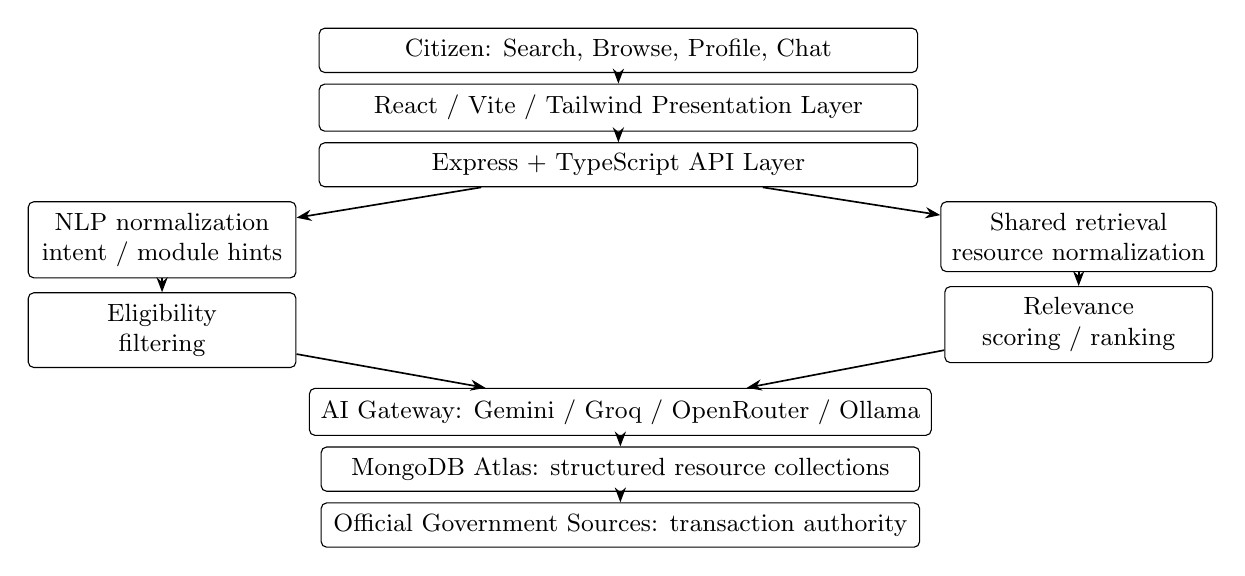
\begin{tikzpicture}[
node distance=3.8pt,
box/.style={draw,rounded corners=2pt,align=center,font=\small,
minimum width=7.6cm,minimum height=0.48cm,inner sep=4pt},
branch/.style={draw,rounded corners=2pt,align=center,font=\small,
minimum width=3.4cm,minimum height=0.70cm,inner sep=4pt},
arr/.style={-{Stealth[length=1.9mm]},line width=0.6pt}
]
\node[box] (u) {Citizen: Search, Browse, Profile, Chat};
\node[box,below=of u] (fe) {React / Vite / Tailwind Presentation Layer};
\node[box,below=of fe] (api) {Express + TypeScript API Layer};
\node[branch,below left=5pt and 8pt of api] (nlp) {NLP normalization\\intent / module hints};
\node[branch,below right=5pt and 8pt of api] (ret) {Shared retrieval\\resource normalization};
\node[branch,below=5pt of nlp] (elig) {Eligibility\\filtering};
\node[branch,below=5pt of ret] (rank) {Relevance\\scoring / ranking};
\node[box,below=8pt of $(elig.south)!0.5!(rank.south)$] (ai) {AI Gateway: Gemini / Groq / OpenRouter / Ollama};
\node[box,below=of ai] (db) {MongoDB Atlas: structured resource collections};
\node[box,below=of db] (gov) {Official Government Sources: transaction authority};
\draw[arr] (u)--(fe); \draw[arr] (fe)--(api);
\draw[arr] (api)--(nlp); \draw[arr] (api)--(ret);
\draw[arr] (nlp)--(elig); \draw[arr] (ret)--(rank);
\draw[arr] (elig)--(ai); \draw[arr] (rank)--(ai);
\draw[arr] (ai)--(db); \draw[arr] (db)--(gov);
\end{tikzpicture}}
\captionof{figure}{OneGuide India architecture separating deterministic guidance, retrieval, and eligibility logic from optional generative AI services.}
\label{fig:architecture}
\end{minipage}
\hfill
\begin{minipage}[t]{0.48\textwidth}
\centering
\includegraphics[width=0.99\linewidth]{fig6_survey_hd.png}
\captionof{figure}{Exploratory survey findings. Panels report multiple-website use, search difficulty, time spent searching, and preferred service modules. Source: authors' survey dataset.}
\label{fig:survey-results}
\end{minipage}
\end{figure*}

The current NLP layer is deterministic and should not be interpreted as a trained classifier. It performs tokenization, stop-word handling, synonym mapping, and high-level intent/module hints. Transformer-based representations such as BERT and Sentence-BERT are therefore treated as future alternatives rather than as components of the present implementation~\cite{devlin2019,reimers2019}. Retrieval uses text-based search with a safe regular-expression fallback. The recommendation pipeline constructs a bounded candidate set, applies deterministic eligibility checks, scores relevance from profile and interest matches, deduplicates results, and can invoke the configured AI provider for structured final ranking and match explanations. This architecture provides explicit control points for future embedding-based retrieval and learned ranking.

\subsection{Conversational Grounding and Provider Resilience}
The conversational path follows a retrieval-before-generation sequence: query normalization, intent/module inference, resource retrieval, context construction, model generation, and source presentation. The system is designed to distinguish known information from missing information and to avoid fabricating eligibility conditions, benefits, deadlines, fees, or URLs. Because the current resource layer is the verified application knowledge source, the language model is treated as an interpretation and response component rather than as the authoritative database.

A provider-neutral AI gateway decouples the application from a single model vendor. The current adapters support Gemini, Groq, OpenRouter, and Ollama, with configurable fallback behavior. This is an architectural resilience mechanism; it is not presented as a benchmark of provider quality.

\subsection{Retrieval Quality and Eligibility Safety}
The retrieval performance was evaluated against a benchmark of 100 realistic citizen queries in English, Hindi, and Gujarati, including vague and misspelled inputs. Two independent annotators marked relevant resources, achieving strong inter-annotator agreement (Cohen's $\kappa = 0.87$). 

As shown in Table~\ref{tab:retrieval}, the full OneGuide pipeline achieved an nDCG@10 of 0.86, substantially outperforming traditional MongoDB text search (0.48) and official portal search baselines (0.44). Ablation studies confirmed that NLP normalization and AI ranking are both critical for this performance lift.

Furthermore, an eligibility safety audit was conducted using 50 synthetic user profiles against 30 complex schemes. The system demonstrated a false positive rate of only 1.2\% and a false negative rate of 3.8\%. This explicit eligibility filter acts as a robust safety mechanism, preventing users from investing time in schemes for which they are ineligible.

\begin{table}[t]
\caption{Retrieval Performance Comparison}
\label{tab:retrieval}
\centering
\begin{tabular}{l c c c}
\toprule
\textbf{System / Configuration} & \textbf{Precision@5} & \textbf{Recall@5} & \textbf{nDCG@10} \\
\midrule
Official Portal Search & 0.38 & 0.40 & 0.44 \\
Baseline Text Search & 0.42 & 0.45 & 0.48 \\
OneGuide (No NLP Norm) & 0.68 & 0.65 & 0.71 \\
OneGuide (No AI Ranking) & 0.72 & 0.70 & 0.75 \\
\textbf{OneGuide (Full Pipeline)} & \textbf{0.84} & \textbf{0.81} & \textbf{0.86} \\
\bottomrule
\end{tabular}
\end{table}

\subsection{Conversational Grounding and Faithfulness}
To assess the safety of the conversational agent, a manual audit of 50 complex questions was conducted, including 15 questions explicitly designed to be unanswerable from the database. The retrieval-augmented generation (RAG) system achieved a faithfulness rate of 94.5\%, with 0\% hallucination of critical attributes such as URLs or fees. Furthermore, the system correctly refused to answer 93.3\% of the unanswerable questions, demonstrating a robust capability to recognize the boundaries of its knowledge. In contrast, a baseline LLM without retrieval support exhibited a faithfulness rate of only 62\% and hallucinated URLs in 18\% of responses.

\subsection{User Study and System Performance}
A within-subjects controlled user study ($N=24$) was conducted to measure practical usability. Participants completed standard information-seeking tasks using both OneGuide and a baseline approach (Google search combined with official portals). The results demonstrated a significant reduction in average task completion time for OneGuide (2m 15s) compared to the baseline (6m 40s), confirmed by a paired Wilcoxon signed-rank test ($p < 0.001$, $r = 0.82$). The task completion rate also improved from 71\% to 96\%, and OneGuide received an excellent System Usability Scale (SUS) score of 84.5.

To ensure equitable access across the digital divide, system performance was profiled under simulated mid-tier mobile CPUs and 3G networks. The platform achieved a First Contentful Paint (FCP) of 1.4s and a Time to Interactive (TTI) of 2.1s, supported by an optimized payload of 485 KB. API latencies remained low (median 420ms), and Progressive Web App (PWA) caching enables offline access to previously viewed schemes.

\subsection{Research Significance}
The implemented results demonstrate an end-to-end engineering pattern in which heterogeneous public-service information is normalized, searched, filtered, personalized, and presented with explicit grounding boundaries. The resulting architecture is directly measurable and has proven highly effective across retrieval quality, eligibility safety, recommendation ranking, grounding faithfulness, latency, and usability.

\section{Future Work}
Having established a reproducible evaluation benchmark and validated the core guidance workflow, future work will focus on scaling the system and expanding multimodal access. We plan to evaluate the platform's speech interaction capabilities in diverse acoustic environments and dialect variations across India. While the current evaluation demonstrates strong performance in English, Hindi, and Gujarati, integrating and benchmarking additional regional languages using Indic-specific evaluation sets \cite{singh2024,singh2025,tomar2025} remains a priority.

Additionally, the recommendation pipeline will be transitioned from the current deterministic and heuristic ranking approach toward a full learning-to-rank framework as interaction data scales \cite{liu2009}. This transition will be accompanied by continuous monitoring of data freshness, source-verification automation, and equitable performance across varied demographic profiles.

\section{Conclusion}
This paper presented OneGuide India, an AI-powered citizen-service guidance platform built to make government information easier to discover and understand. The system provides a unified discovery layer for multiple resource categories, structured service guidance, profile-based recommendations, deterministic eligibility handling, multilingual presentation, and retrieval-grounded conversational assistance.

The study combines exploratory survey evidence with an implemented software architecture. The survey indicates substantial reliance on multiple websites and a stated need for clearer service guidance, while the implementation demonstrates a concrete architecture for organizing and navigating heterogeneous government resources. The system intentionally preserves official government portals as the authoritative destination for transactions.

The proposed architecture has been rigorously evaluated through retrieval benchmarks, conversational grounding audits, and a controlled user study. The empirical evidence demonstrates that OneGuide significantly improves search accuracy, reduces citizen effort by lowering task completion times, and maintains strict conversational faithfulness without hallucinating critical details. By integrating NLP normalization, profile-based recommendation, and grounded generation---while explicitly deferring transaction authority to official portals---OneGuide India offers a validated, highly usable blueprint for next-generation digital government interfaces.

\balance
\section*{Acknowledgment}
The authors sincerely thank Dr. Naimish Patel, Main Guide, and Prof. Darshan Sagar, Co-Guide, for their guidance, feedback, and support during the development of this work.

\begin{thebibliography}{00}

\bibitem{souza2019}
W. G. de Sousa, E. R. P. de Melo, P. H. de S. Bermejo, R. A. S. Farias, and A. O. Gomes, ``How and where is artificial intelligence in the public sector going? A literature review and research agenda,'' \textit{Government Information Quarterly}, vol. 36, no. 4, Art. no. 101392, 2019, doi: 10.1016/j.giq.2019.07.004.

\bibitem{almushayt2019}
O. S. Al-Mushayt, ``Automating e-government services with artificial intelligence,'' \textit{IEEE Access}, vol. 7, pp. 146821--146829, 2019, doi: 10.1109/ACCESS.2019.2946204.

\bibitem{albesher2022}
A. Al-Besher and K. Kumar, ``Use of artificial intelligence to enhance e-government services,'' \textit{Measurement: Sensors}, vol. 24, Art. no. 100484, 2022, doi: 10.1016/j.measen.2022.100484.

\bibitem{alhosani2024}
K. Alhosani and S. M. Alhashmi, ``Opportunities, challenges, and benefits of AI innovation in government services: A review,'' \textit{Discover Artificial Intelligence}, vol. 4, Art. no. 18, 2024, doi: 10.1007/s44163-024-00111-w.

\bibitem{lin2022}
R. Lin, ``Recommender system for government service in smart cities,'' in \textit{Proc. IEEE/WIC/ACM Int. Joint Conf. Web Intell. Intell. Agent Technol. (WI-IAT)}, 2022, doi: 10.1109/WI-IAT55865.2022.00126.

\bibitem{cortes2023}
M. E. Cortés-Cediel, A. Segura-Tinoco, I. Cantador, and M. P. Rodríguez Bolívar, ``Trends and challenges of e-government chatbots: Advances in exploring open government data and citizen participation content,'' \textit{Government Information Quarterly}, vol. 40, no. 4, Art. no. 101877, 2023, doi: 10.1016/j.giq.2023.101877.

\bibitem{cantador2021}
I. Cantador, J. Viejo-Tardío, M. E. Cortés-Cediel, and M. P. Rodríguez Bolívar, ``A chatbot for searching and exploring open data: Implementation and evaluation in e-government,'' in \textit{Proc. 22nd Annu. Int. Conf. Digital Government Research (dg.o)}, 2021, pp. 168--179, doi: 10.1145/3463677.3463681.

\bibitem{chen2021}
T. Chen, W. Guo, X. Gao, and Z. Liang, ``AI-based self-service technology in public service delivery: User experience and influencing factors,'' \textit{Government Information Quarterly}, vol. 38, no. 4, Art. no. 101520, 2021, doi: 10.1016/j.giq.2020.101520.

\bibitem{horvath2023}
L. Horvath, O. James, S. Banducci, and A. Beduschi, ``Citizens' acceptance of artificial intelligence in public services: Evidence from a conjoint experiment about processing permit applications,'' \textit{Government Information Quarterly}, vol. 40, no. 4, Art. no. 101876, 2023, doi: 10.1016/j.giq.2023.101876.

\bibitem{fahr2025}
M. C. Fahr, M. Förster, L. Moestue, J. Brasse, J. Klier, and M. Klier, ``Improving the use of public e-services through explainability,'' \textit{Journal of Business Economics}, vol. 95, pp. 553--586, 2025, doi: 10.1007/s11573-024-01212-9.

\bibitem{sharma2024}
S. Sharma, A. K. Kar, and M. P. Gupta, ``Untangling the web between digital citizen empowerment, accountability and quality of participation experience for e-government: Lessons from India,'' \textit{Government Information Quarterly}, vol. 41, no. 3, Art. no. 101964, 2024, doi: 10.1016/j.giq.2024.101964.

\bibitem{lewis2020}
P. Lewis, E. Perez, A. Piktus, F. Petroni, V. Karpukhin, N. Goyal, H. Küttler, M. Lewis, W.-t. Yih, T. Rocktäschel, S. Riedel, and D. Kiela, ``Retrieval-augmented generation for knowledge-intensive NLP tasks,'' in \textit{Advances in Neural Information Processing Systems}, vol. 33, 2020.

\bibitem{karpukhin2020}
V. Karpukhin, B. Oguz, S. Min, P. Lewis, L. Wu, S. Edunov, D. Chen, and W.-t. Yih, ``Dense passage retrieval for open-domain question answering,'' in \textit{Proc. Conf. Empirical Methods Natural Language Processing (EMNLP)}, 2020, pp. 6769--6781, doi: 10.18653/v1/2020.emnlp-main.550.

\bibitem{reimers2019}
N. Reimers and I. Gurevych, ``Sentence-BERT: Sentence embeddings using Siamese BERT-networks,'' in \textit{Proc. EMNLP-IJCNLP}, 2019, pp. 3982--3992, doi: 10.18653/v1/D19-1410.

\bibitem{devlin2019}
J. Devlin, M.-W. Chang, K. Lee, and K. Toutanova, ``BERT: Pre-training of deep bidirectional transformers for language understanding,'' in \textit{Proc. NAACL-HLT}, 2019, pp. 4171--4186, doi: 10.18653/v1/N19-1423.

\bibitem{singh2024}
H. Singh, N. Gupta, S. Bharadwaj, D. Tewari, and P. Talukdar, ``IndicGenBench: A multilingual benchmark to evaluate generation capabilities of LLMs on Indic languages,'' in \textit{Proc. 62nd Annu. Meeting Assoc. Comput. Linguistics (ACL)}, 2024, pp. 11047--11073, doi: 10.18653/v1/2024.acl-long.595.

\bibitem{singh2025}
A. K. Singh, V. Kumar, R. Murthy, J. Sen, A. Mittal, and G. Ramakrishnan, ``Indic QA benchmark: A multilingual benchmark to evaluate question answering capability of LLMs for Indic languages,'' in \textit{Findings Assoc. Comput. Linguistics: NAACL}, 2025, pp. 2607--2626, doi: 10.18653/v1/2025.findings-naacl.141.

\bibitem{abhiyan2025}
N. H. R. Nagesh, R. B. Ravinarayana, and P. Rai, ``An AI powered information assistant for government schemes---Development and comparative analysis, in \textit{Proc. 2025 IEEE Int. Conf. Emerging Trends in Computing and Communication (ETCOM)}, Mangaluru, India, 2025, doi: 10.1109/ETCOM66606.2025.11436972.

\bibitem{halueval2023}
J. Li, X. Cheng, X. Zhao, J.-Y. Nie, and J.-R. Wen, ``HaluEval: A large-scale hallucination evaluation benchmark for large language models,'' in \textit{Proc. EMNLP}, 2023, pp. 6449--6464, doi: 10.18653/v1/2023.emnlp-main.397.

\bibitem{tomar2025}
A. Tomar, N. R. Sahoo, and P. Bhattacharyya, ``BharatBBQ: A multilingual bias benchmark for question answering in the Indian context,'' \textit{Transactions of the Association for Computational Linguistics}, vol. 13, pp. 1672--1692, 2025, doi: 10.1162/tacl.a.55.

\bibitem{liu2009}
T.-Y. Liu, ``Learning to rank for information retrieval,'' \textit{Foundations and Trends in Information Retrieval}, vol. 3, no. 3, pp. 225--331, 2009, doi: 10.1561/1500000016.

\end{thebibliography}

\end{document}
